\ifx\wholebook\relax \else

\documentclass[b5paper]{article}
\usepackage[nomarginpar
  %, margin=.5in
]{geometry}

\addtolength{\oddsidemargin}{-0.05in}
\addtolength{\evensidemargin}{-0.05in}
\addtolength{\textwidth}{0.1in}

\usepackage[en]{../prelude}

\setcounter{page}{1}

\begin{document}

\title{Numerals}

\author{Xinyu LIU
\thanks{{\bfseries Xinyu LIU} \newline
  Email: liuxinyu99@hotmail.com \newline}
  }

\maketitle
\fi

\markboth{Numerals}{A tour of numbers}

\ifx\wholebook\relax
\chapter{Numerals}
\fi

\epigraph{The total number of minds in the universe is one.}{Erwin Schrödinger}

Numbers appear everywhere in our life. For example, this news: \enquote{\textit{The 2024 Paris Olympic Games to an end on Sunday August 11, 2024. Paris is the second city, after London, to host the Summer Olympics three times. It set a record of gender equality, with 5,250 male and 5250 female athletes. In total, 32 sports and 329 events were featured, with 206 countries and regions participating. Four new sports made their debut: skateboarding, surfing, sport climbing, and breakdancing. A total of 329 gold medals were up for grabs. Athletes from various countries and regions demonstrated outstanding athleticism. The United States and China tied for the most gold medals, with each securing 40. The United States also led in silver medals with 44 and bronze medals with 42.}} It contains 14 numbers among the total of 120 words. We don't know who invented the numerals because they show up in almost all historic documents to the very early time. Some believe numerals arose with language. Anthropologists identified numbers inscribed in bones, stones, caves, clay, etc. We can also find such clues in our languages, for example in English, eleven comes from `endleofan', meaning (ten) left one; twelve comes from `twelf', meaning left two.

\section{Rosetta stone}
\index{Rosetta stone}  \label{sec:rosetta-stone}

\begin{figure}[htbp]
 \centering
 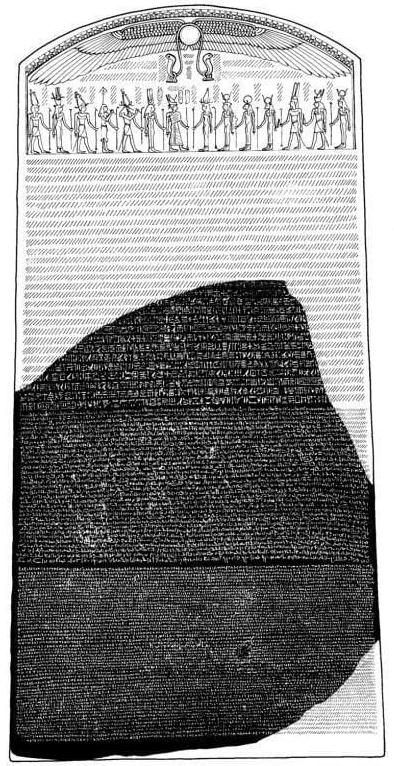
\includegraphics[scale=0.5]{img/Rosetta-stone-recons}
 \caption{Rosetta stone is broken in the middle.}
 \label{fig:rosetta-stone-recons}
\end{figure}

There is a famous object in room 4 of the British museum, the Rosetta stone. It's a broken inscribed stela with the length of 112cm, the width of 76cm (figure \ref{fig:rosetta-stone-recons}). One can identifies some Greek characters like \cref{fig:rosetta-greek} (see \cref{tab:greek-alphabet} of Greek alphabet) in the bottom, while the remaining are mystery ancient characters. When read carefully, there are two different types: a curved form as in \cref{fig:rosetta-demotic} in the middle of the stone, and some small pictures as in \cref{fig:rosetta-hieroglyphs} on the top.

\begin{figure}[htbp]
  \centering
  \subcaptionbox{54 lines in Ancient Greek.\label{fig:rosetta-greek}}{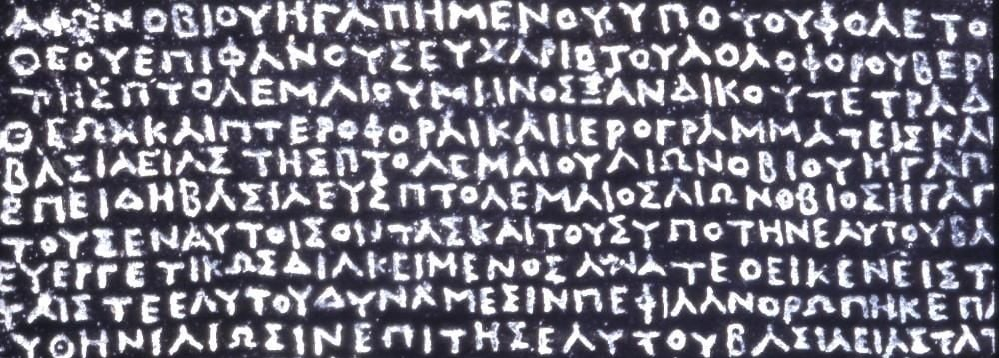
\includegraphics[scale=0.5]{img/Rosetta-Greek}} \\
  \subcaptionbox{32 lines in Demotic, a cursive form of Hieroglyphics use for ordinary document.\label{fig:rosetta-demotic}}{\quad 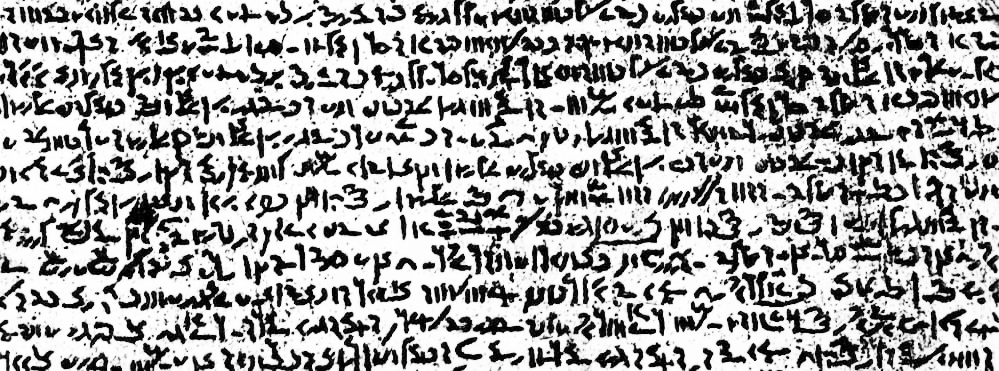
\includegraphics[scale=0.5]{img/Rosetta-Demotic}\quad} \\
  \subcaptionbox{14 lines in Hieroglyphic, the script most used for religious texts.\label{fig:rosetta-hieroglyphs}}{\qquad 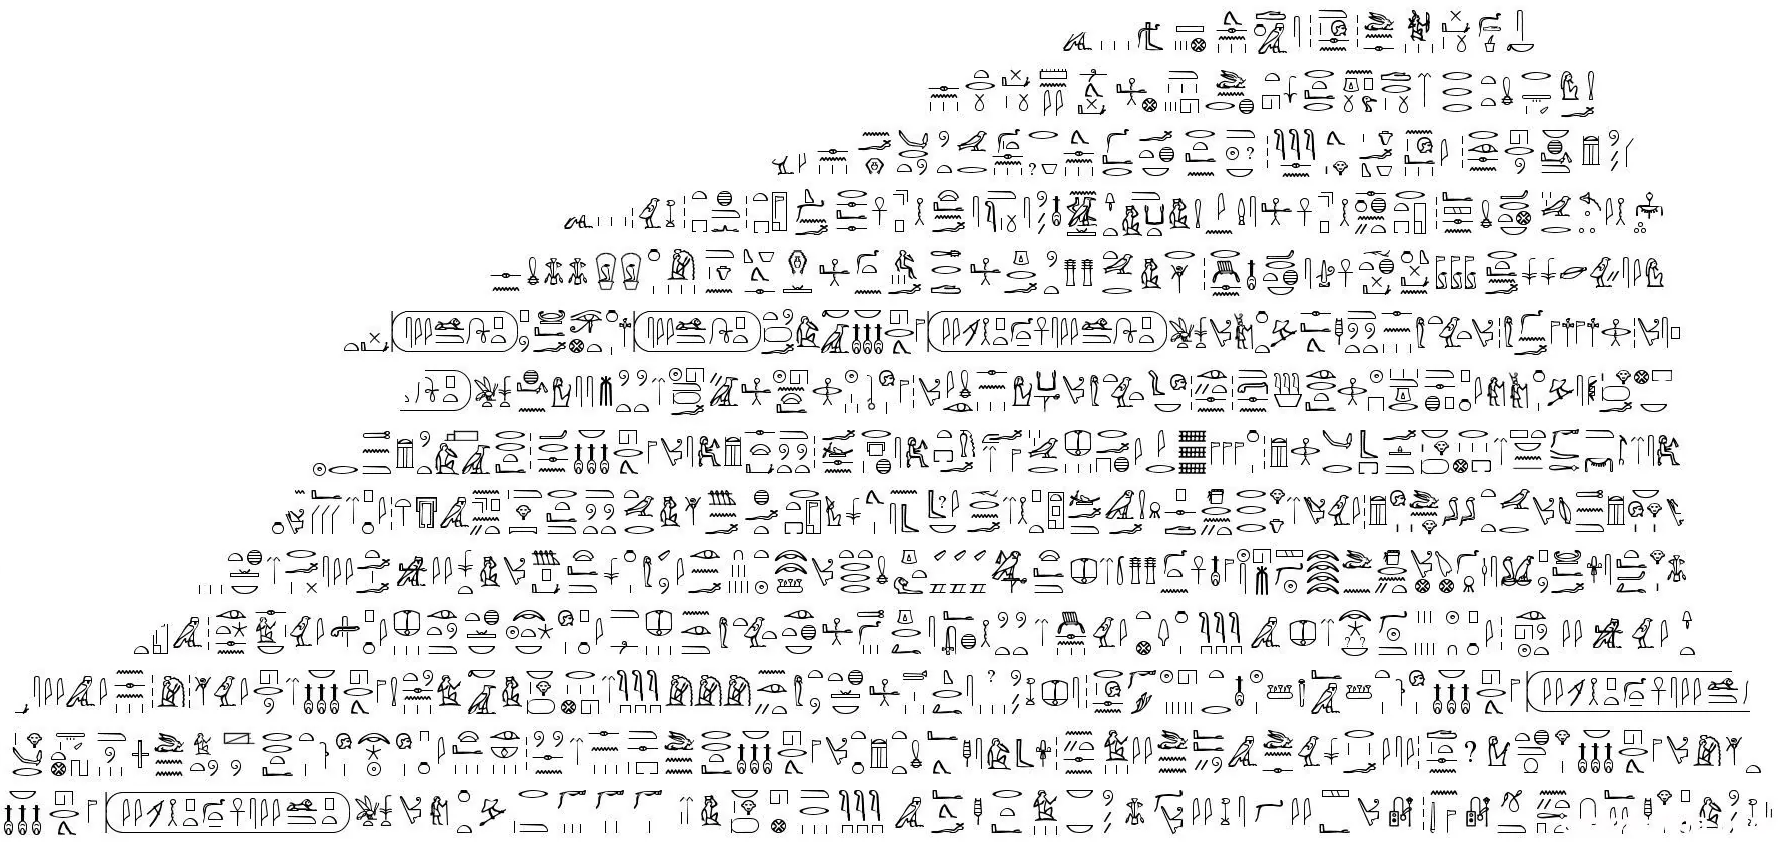
\includegraphics[scale=0.3]{img/Rosetta-Hieroglyphs-c}\qquad}
  \caption{Three different scripts and languages on Rosetta stone.}
  \label{fig:rosetta-stone}
 \end{figure}

The discovery of the Rosetta stone was during the expedition when Napoleon Bonaparte campaigned in Egypt from 1798 to 1701, aimed to establish a colony in Egypt and to threaten British possessions in India. The French troop had about 3,800 soldiers, a fleet of 326 ships, and 167 most distinguished scientists and scholars directed by mathematician Gaspard Monge\cite{Harrison-2023}. This gave the expedition a scientific purpose, to conduct research and show off scientific advances. The fleet secretly sailed from Toulon, and lucky by-passed the British Royal Navy's detection in thick fog. Napoleon's army captured Alexandria on 2 July, then set out for Cairo. On 16 July 1799, Some French soldiers accidentally discovered the Rosetta stone when digging the foundations of an addition to a fort near the town of Rosetta in the Nile Delta. It had apparently been built into a very old wall. Although the stone was broken, it was an important discovery. The officer sent it to the Egypt research center founded by Napoleon in Cairo in August. It was named after Rosetta, the discovered place. After the French surrender of Egypt in 1801, it passed into British hands. The stone was shipped to England and arrived in Portsmouth in February 1802. It is now in the British Museum in London.

What makes this stone important is its inscription. It's a decree in three different scripts: Hieroglyphs (suitable for a priestly decree), Demotic (the cursive Egyptian script used for daily purposes, meaning `language of the people'), and ancient Greek. It's about the affirmation to the royal cult of the 13 years old Ptolemy V on the first anniversary of his coronation (in 196 BCE), saying he inherited the legitimate throne from his father, Ptolemy IV, and carried out many good deeds, such as donating to temples, exempting taxes, and so on. The rulers of Egypt at this point were Greco-Macedonian after Alexander the Great's conquest\footnote{Ptolemy I, a Macedonian general of Alexander the Great, became the ruler of Egypt in 305 BCE. He founded the Ptolemaic dynasty which last for 275 years.}. The Macedonian king of Egypt was also the pharaoh, hence the decree was inscribed in ancient Greek as the official language besides Hieroglyphs and Demotic. It was copied on to large stones, which were put in every temple in Egypt. Rosetta stone is one and the only one ever discovered of these copies\footnote{Another limestone memorial plaque with three inscriptions in Roman period (30 BCE - 295 AD) was discovered in 1913 near a temple in Egypt. There left 4 lines of Hieroglyphs, 7 lines of Demotic, and 7 lines of ancient Greek from top to bottom. Similar to the Rosetta stone, the top part was badly broken and incomplete\cite{SH-Museum-24}.}. The Rosetta Stone became a valuable key to deciphering the hieroglyphs because the inscriptions say the same thing in three different scripts, and scholars could still read ancient Greek. Thomas Young (1773 - 1829)\footnote{The English physicist who established the principle of interference of light and thus resurrected the century-old wave theory of light.}, an English Physicist and the French scholar Jean-François Champollion (1790 - 1832) successfully established an entire list of signs with their Greek equivalents based on study of the Rosetta stone, their work enabled us to read Egyptian hieroglyphic texts\cite{BM-RS-17}.

\section{Ancient Egyptian numerals and Babylonian numerals}
\index{numeral system}

The numeral symbols appeared in ancient Egypt as early as 3400 BCE. It's the earliest in the world (about 3000 BCE in Mesoputamia; about 1600 BCE in ancient China\cite{Clawson-1994}). The initial symbols were typical `|', `||', `|||' or `—', `=', `$\equiv$' and so on. Our ancestors seemed to start from counting, for example, to count the hunted animals or collected fruits. It appears people count with fingers at first; gradually, they counted to 10 and need bigger numbers. However, human only has two hands of 10 fingers. There are three ways to solve the insufficiency: (1) with the help of feet, we can count to 20, and then meet the same issue again; (2) Free grouping, for example, the Yukaghirs of Siberia counted, ``three and one, two threes, two threes and one, two fours, ten with one missing.'' (3) Fixed grouping, when count to a fixed number, e.g., 10, treat the group of things as a unit; and name it with a special symbol. For example, ancient Egyptian used $\cap$ to represent 10, hence, $\cap \cap$ means 20 (ancient Roman represented 10 as X, 1 as I, hence 23 is XXIII, consisted of two Xs and three Is).

\begin{figure}[htbp]
 \centering
 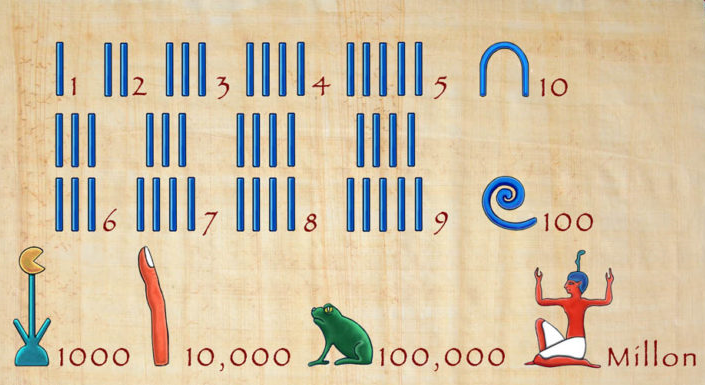
\includegraphics[scale=0.8]{img/hieroglyphic-numbers}
 \caption{Hierogyphic numerals in ancient Egypt.}
 \label{fig:egypt-hieroglyphic-numerals}
\end{figure}

\index{ancient Egypt numerals}
To build the great pyramid, ancient Egyptian created many symbols for big numbers, as shown in \cref{fig:egypt-hieroglyphic-numerals}. They used the symbol of Heh, the god of infinity in Egyptian religion, to represent a million; a tadpole for 100,000; a finger for 10,000; a lotus for a thousand; a rope for a hundred. Repeated grouping when count numbers, if exceeded then grouped to higher level of unit. The value of such a number is the sum of the products of the unit and digit. \Cref{fig:egypt-number-examples} shows two examples.

\begin{figure}[htbp]
 \centering
 \subcaptionbox{212427 is $2(100,000)+1(10,000)+2(1,000)+4(100)+2(10)+7(1)$}{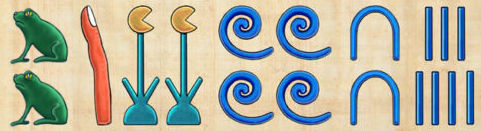
\includegraphics[scale=0.5]{img/egypt-num-eg2}}
 \subcaptionbox{The number, 1,333,330, is inscribed in Edfu temple in Egypt.}{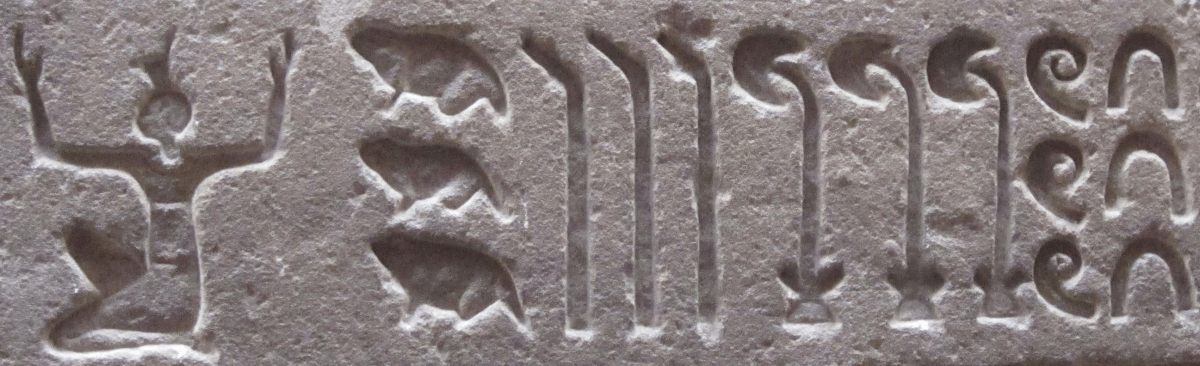
\includegraphics[scale=0.2]{img/Hieroglyphic-num-eg}}
 \caption{Egyptian numbers}
 \label{fig:egypt-number-examples}
\end{figure}

\index{Babylonian numerals} \index{sexagesimal} \index{cuneiform}
Although method (3) can handle big numbers, method (2) is convenient for small numbers. Ancient Babylonians lived in Mesopotamia. The name of the region comes from a Greek word, meaning `between rivers'. It refers to the center of the land between Tigris and Euphrates rivers (in Iraq nowadays). The people impressed their symbols in damp clay tablets. After drying in the sun or in a kiln, the tablets became as permanent as stone. Because the symbol given by the stylus is wedge-shaped, the inscriptions are known as cuneiform\footnote{Combined from `wedge' (cuneus in Latin) and `shape' (forma in Latin).}. Ancient Babylonians used sexagesimal (base 60) system, which is partly left today. For example, a minute has 60 seconds; an hour has 60 minutes. An hour 12 minutes and 30 seconds is written as 1:12:30, which equals $1(60\times 60) + 12(60) + 30 = 4350$ seconds. 60 is not a small number, it appears Babylonians used a mixed system in practical: grouped with 10 for numbers less than 60, otherwise, grouped with $60^2$、$60^3$、$60^4, \dotsc$. \Cref{fig:babylonian-numerals} shows the cuneiform symbols from 1 to 59. We can easily see the pattern: a vertical wedge (Y) for number 1, add such a wedge for each number from 2 to 9; a horizontal wedge (<) for 10, from 11 to 19, the number is a horizontal wedge (10) plus the corresponding vertical wedges. Two horizontal wedges for 20, then repeated the rule within 60, i.e., 10 times the number of horizontal wedges plus the number of vertical wedges.

\begin{figure}[htbp]
 \centering
 \subcaptionbox{Numbers from 1 to 59 in Babylonia.\label{fig:babylonian-numerals}}{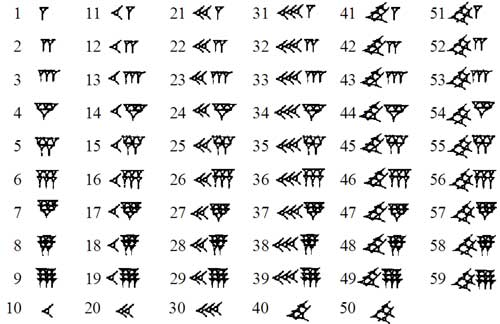
\includegraphics[scale=0.8]{img/Babylonian-numerals}} \\
 \subcaptionbox{Example: $1(60^3) + 19(60^2) + 21(60) + 54$\label{fig:babylonian-num-eg}}{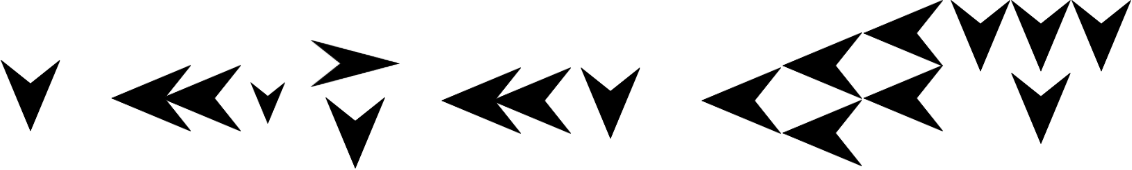
\includegraphics[scale=0.2]{img/Babylonian-num-eg}}
 \caption{Ancient Babylonian numerals.}
\end{figure}

\index{Positional numeral system}
However, numbers greater than 60 have different pattern, as shown in \cref{fig:babylonian-num-eg}. 285714 is 1:19:21:54 in sexagesimal format, but 19 was written as $20 - 1$, where the small vertical wedge means minus. The number being subtracted is annotated with a wedge pointed to right. Evidently, this is not strictly our 60-based number today, but a mixed one with subtraction within 60. Different from Egyptian, Babylonian didn't create dedicated symbols for $60, 60^2, 60^3, \dotsc$; the value of a digit is determined by its position. The left most is the number of 1s, the second is the number of units of 60, the third is the numbe of units of $60^2$, and so on. This is called the positional system. However, Babylonian numbers might have ambiguity because lack of zero. Actually, they invented a symbol for empty place about 300 BCE, but it was used only in the middle of a number but not at the end. As a result, we can't distinguish between 11 and 1100; The later translators suffer from this problem and have to guess from the context.

\section{Roman numerals and Chinese numerals}
\index{Multiplicative grouping system} \index{Roman numerals}

Roman numerals have strong influence still today as the arising of the Roman civilization across Europe, Africa, and Asia. We still see Roman numbers in clocks (see \cref{fig:clock-plate}), buildings, table of content of books. It's easy for memorize as there are only few letters: I, V, X, C, and M. It's convenient to represent small numbers, such as III for 3, VII for 5 (= 2 + 7). 2025 which is MMXXV contains two 1000, two 10, and 5. However, there are so many ways to represent a number, that brings big confusion to decipher. At the beginning, people only needed to sum up the numbers of each letter, but then came the rule of `subtracting on the left and adding on the right'. For example, IV means $5 - 1 = 4$, but VI means $5 + 1 = 6$. Hence IXX $= (10 - 1) + 10 = 19$, while $19 = 10 + (10 - 1) =$ XIX causes ambiguity, because XIX can also be interpreted as (XI)X = 11 + 10 = 21. Similarly, XVIII = 16, but then both $16 = 8 + 8 =$ IIXIIX and $16 = (10 - 4) + 10 =$ IIIIXX have ambiguity. Where IIIIXX for 88 appeared in a Pairs treaty of 1388\cite{LeVeque-Smith-25}.

\btab{|c|c|c|c|c|}
\hline
1 & 5 & 10 & 100 & 1000 \\
\hline
I & V & X  & C   & M \\
\hline
\etab

\begin{figure}[htbp]
 \centering
 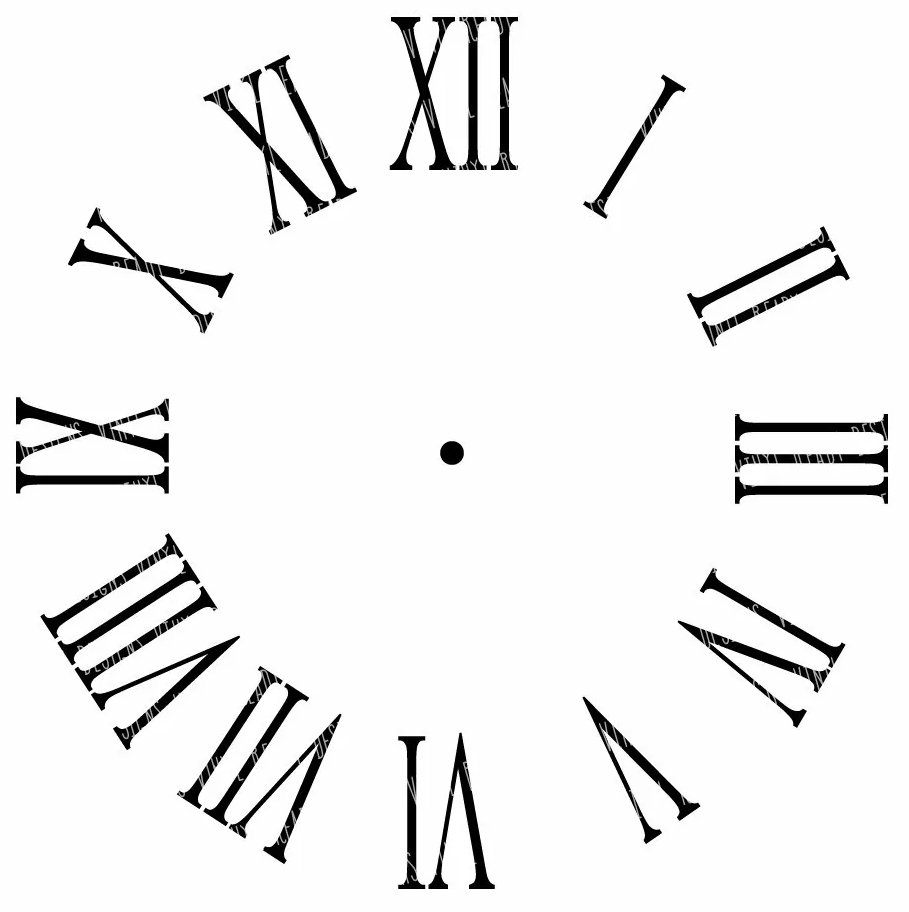
\includegraphics[scale=0.4]{img/clock-plate}
 \caption{Roman numerals in clock plate}
 \label{fig:clock-plate}
\end{figure}

\index{ancient Chinese numerals}
Ancient Chinese numerals are decimal based multiplicative grouping system, which is quite close to the modern numerals. The first 10 characters are:

\begin{center}
\begin{tabular}{cccccccccc}
{一} & {二} & {三} & {四} & {五} & {六} & {七} & {八} & {九} & {十} \\
\end{tabular}
\end{center}

In English eleven comes from (ten) left one, and twelve comes form (ten) left two; such things didn't happen in Chinese. The next numbers are {十一} (ten and one), {十二} (ten and two) ... {十九} (ten and nine), then {二十} (two of ten) ... {九十九} (nine of ten and nine). There are special symbols like {廿} for 20 and {卅} for 30, often appear in calendar. The greater decimal group symbols are {百} (hundred), {千} (thousand), and {万} (1000). For example 6147 is written as {六千一百四十七 (6千1百4十7)}, which can be understood as 6M1C4X7I with Roman symbols. The value is the sum of product of each digit and unit. It looks almost as same as the modern numerals, but there is difference. There was no symbol of zero until the 11th century, then a character was reused as zero\footnote{This character has the meaning of rain in ancient time. We don't find it in {\em Nigh chapters on the Art of mathematics}, a classic Chinese mathematical book around 1st century CE in Han dynasty.}. However, zero isn't strictly used even today (also in English), for example 108 is read as a hundred and eight (一百単八\footnote{A popular number comes from the novel {\em All Men Are Brothers} in 14th century.}), but not a hundred, zero ten, and eight. It causes ambiguity as Chinese people sometimes say a hundred eight (一百八) to mean 180 but not 108. Without zero, people need name every unit of group. More symbols were created for greater numbers, but there are finite many symbols while number can increase infinitely. \Cref{tab:units-en} and \cref{tab:units-en} list English and Chinese units.

\index{units}
\begin{table}[htbp]
  \centering
  \begin{tabular}{|l|r|l|r|l|r|}
  \hline
  thousand & $10^{3}$ & duodecillion  & $10^{39}$ & quattuorvigintillion & $10^{75}$ \\
  \hline
  million & $10^{6}$ & tredecillion  & $10^{42}$ & quinvigintillion & $10^{78}$ \\
  \hline
  billion & $10^{9}$ & quattuordecillion & $10^{45}$ & sexvigintillion & $10^{81}$ \\
  \hline
  trillion  & $10^{12}$ & quindecillion & $10^{48}$ & seprvigintillion & $10^{84}$ \\
  \hline
  quadrillion  & $10^{15}$ & sexdecillion & $10^{51}$ & octovigintillion & $10^{87}$ \\
  \hline
  quintillion  & $10^{18}$ & septdecillion & $10^{54}$ & novemvigintillion & $10^{90}$ \\
  \hline
  sexillion    & $10^{21}$ & octodecillion & $10^{57}$ & trigintillion & $10^{93}$ \\
  \hline
  septillion   & $10^{24}$ & novemdecillion & $10^{60}$ & untrigintillion & $10^{96}$ \\
  \hline
  octillion    & $10^{27}$ & vigintillion & $10^{63}$ & duotrigintillion & $10^{99}$  \\
  \hline
  noniliion  & $10^{30}$ & unvigintillion & $10^{66}$ & googol & $10^{100}$ \\
  \hline
  decillion  & $10^{33}$ & duovigintillion & $10^{69}$ & & \\
  \hline
  undecillion   & $10^{36}$ & trevigintillion & $10^{72}$ & & \\
  \hline
  \end{tabular}
  \caption{English units}
  \label{tab:units-en}
\end{table}

The last unit in English, googol, was coined in 1920 by 9-year-old Milton Sirotta, nephew of U.S. mathematician Edward Kasner. It is digit 1 followed by one hundred zeros. The internet company Google’s name comes from this word.

\begin{table}[htbp]
  \centering
  % for Pinyin tones: \={a}, \'{a}, \v{}, \.{a}
  \begin{tabular}{|l|r|l|r|l|r|}
  \hline
  百            & $100$      & 秭(z\v{i})    & $10^{24}$ &  恒河沙  & $10^{52}$ \\
  \hline
  千            & $1000$     & 穰(r\'{a}ng)  & $10^{28}$ & 阿僧祗(zh\={i})  & $10^{56}$ \\
  \hline
  万            & $10000$    & 沟            & $10^{32}$ & 那由他        & $10^{60}$  \\
  \hline
  億            & $10^8$     & 澗            & $10^{36}$ &  不可思議      & $10^{64}$ \\
  \hline
  兆            & $10^{12}$  & 正            & $10^{40}$ &  无量大数      & $10^{68}$ \\
  \hline
  京            & $10^{16}$  & 載            & $10^{44}$ &               & \\
  \hline
  垓(g\={a}i)   & $10^{20}$  & 极            & $10^{48}$ &               & \\
  \hline
  \end{tabular}
  \caption{Chinese units}
  \label{tab:units-cn}
\end{table}

Many Chinese units come from Buddhism\cite{Noguchi2007}, like 恒河沙, means the sand-grain in Ganges River. It has 52 zeros after 1. Starting from one, there is a unit for every 10,000 magnitude in Chinese (compare to 1000 magnitude step in English).

\section{Positional numeral system}
\index{positional numeral system} \index{Mayan numeral system} \index{solar year}

During early expedition to Yucatán Peninsula (in the central America between the Gulf of Mexico and the Caribbean Sea), the Spanish discovered Maya civilization. They had a well-developed numeral system as shown in \cref{fig:maya-numerals}. Similar to Babylonian 10-60 mixed base system, Mayan had a 5-20 mixed base system. For numbers less than 20, they were 5-based. A dot represented one; two dots for tow; drew a line every time counted to five till 20; then switch to 20-based. They wrote vertically and had a special symbol for zero. It seems that Mayan numerals were used primarily for the calendar. Taking 20 days per month, Mayan found $20 \times 18 = 360$ was close to a solar year. They arranged 18 months with 5 `nameless' days (called Uayeb means unlucky days) setting a year of 365 days. Then added an extra day every 4 years to offset the error. This is almost same as our present definition of a solar year.

\begin{figure}[htbp]
 \centering
 \subcaptionbox{5-based within 20}{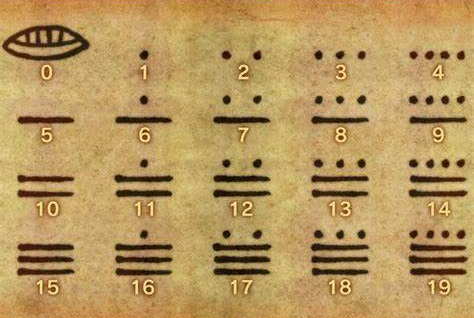
\includegraphics[scale=0.9]{img/Maya-numerals}}
 \subcaptionbox{$2(20^3) + 0(20^2) + 6(20) + 13 = 16133$}{\qquad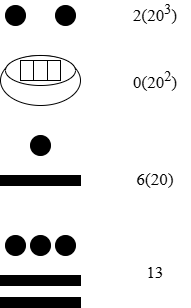
\includegraphics[scale=0.4]{img/Maya-num-eg}\qquad}
 \caption{Mayan numerals}
 \label{fig:maya-numerals}
\end{figure}

Neither Mayan 20-based system nor Babylonian 60-based system needs names for grouping unit, but relies on the position to indicate the magnitude of a digit. It's called {\em positional numeral system}, which satisfies three criteria:

\begin{enumerate}[1)]
\item A base $b$, for example $b = 10$ in our decimal numbers; $b = 60$ in Babylonian numbers; $b = 20$ in Mayan numbers.
\item Give names to $1, 2, \cdots, b-1$. For example, one, two, three, ..., nine in English; 一, 二, 三, ..., 九 in Chinese; a dot, two dots, ..., 4 dots and a line in Mayan.
\item A symbol of zero.
\end{enumerate}

Any number $n$ in a positional numeral system equals to:

\be
n = a_m b^m + a_{m-1} b^{m-1} + \cdots + a_a b + a_0
\label{eq:pos-rep}
\ee

where $a_i$ is the named digit for $0, 1, 2, \cdots, b-1$. $n$ is written as $a_ma_{m-1} \cdots a_0$. For example, $2024 = 2 \times 10^3 + 0 \times 10^2 + 2 \times 10 + 4$, where $b = 10, m = 3, a_3 = 2, a_2 = 0, a_1 = 2, a_0 = 4$, written exactly as 2024. Note that 0 acts the key role to `occupy' a position: There are 2 thousand, 2 ten, 4 one, but no hundred. because 0 occupies the place of hundred, every digit has the right magnitude. Otherwise, the number would be 224 incorrectly.

\begin{example}
In the kingdom of cat, octal numerals are used because a cat has four `fingers' each paw (see \cref{fig:cat-paw}, total 8 fingers with two paws. They use `mew' as zero; the numbers from 1 to 7 in this kingdom are: (1) miao, (2) mieo, (3) meio, (4) meow, (5) miuo, (6) meao, and (7) meeo. There are $365 = 5 \times 64 + 5 \times 8 + 5$ days in a year, which is `miuo miuo miuo'. Year $2024 = 5 \times 8^3 + 3 \times 8^2 + 7 \times 8 + 0$ is `miuo meio meeo mew'.

\begin{figure}[htbp]
 \centering
 
\includegraphics[scale=0.6]{img/cat-paw}
 \caption{Cat paw}
 \label{fig:cat-paw}
\end{figure}

\end{example}

\begin{example}
\index{hexadecimal}
Programmers often use hexadecimal (16-based) system. Numbers 0, 1, ..., 9 are reused, followed with A, B, C, D, E, F to represent 10 to 15. A year of 365 days is decomposed to $365 = 1 \times 16^2 + 6 \times 16 + 13$, which is 16D in hexadecimal. $2024 = 7 \times 16^2 + 14 \times 16 + 8$, which is 7E8 in hexadecimal.
\end{example}

One big issue with Roman numbers is ambiguity; there are multiple ways to write a number and different numbers may share the same written form. Can it be solved by positional system? Of course we see 8 = 08 = 008 in elevator, digital clock, and odometer. The value keeps unchanged when adding zeros to the left. Let's rule out this case, assume $a_m \ne 0$ in \cref{eq:pos-rep}, then the positional representation is unique for any number (see \cref{qn:unique-pos-rep}).

%
\begin{figure}[htbp]
 \centering
 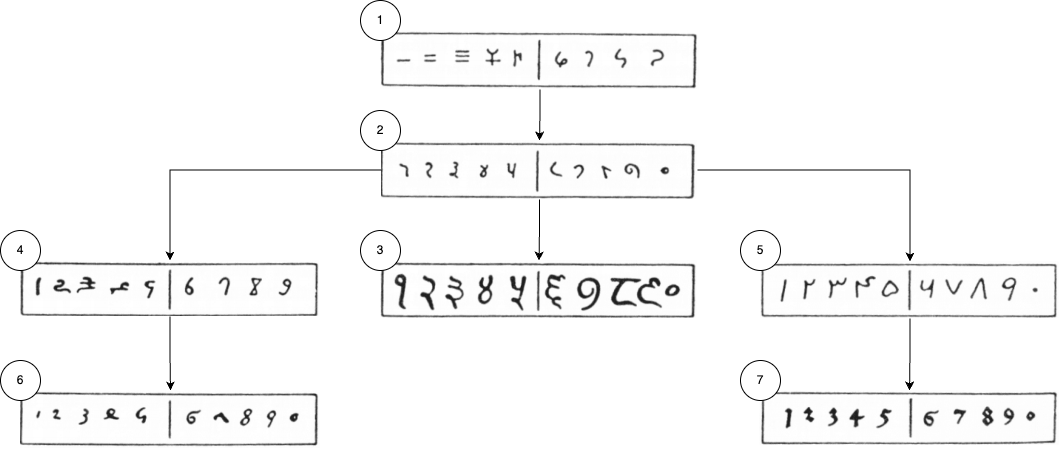
\includegraphics[scale=0.3]{img/Hindu-arabic-num}
 \caption{Hindu-Arabic numerals: (1) Brahmi, 1st century CE, (2) Indian (Gwalior), 9th century, (3) Sanskrit Davanagari, Indian, 11th Cenntury, (4) West Arabic (Gubar or Gobar), 11th century, (5) East Arabic, 11th century, (still used in Turkey), (6) 15th century, (7) 16th century (Dürer)}
 \label{fig:hindu-arabic-numerals}
\end{figure}

\index{Hindu-Arabic numeral system} \index{zero} \index{Brahmagupta} \label{sec:hindu-arabic-numerals}
Both Babylonian and Mayan numerals disappeared. They didn't suit for computations, for the digits less than 20 or 60 were not represented by single symbols, and the mixed base is complex. Our present positional numeral system was developed by Hindus and brought to western through the hand of Arabic. It's called the Hindu-Arabic system. The symbol of 1, 4, and 6 appeared in the Ashoka inscriptions around 3rd century BCE; then 2, 3, 4, 5, 6, 7, 9 appeared in the Nasik caves of 1st or 2nd century CE. We can see the clue that 2 came from `$=$' and 3 came from `$\equiv$'. Although Indian mathematician Brahmagupta defined zero in the 7th century \cite{MacTutor-Brahmagupta-2000}, but we haven't seen the symbol 0 until the 9th century (see \cref{fig:hindu-arabic-numerals}). Hindus used a dot or a small circle for zero at first, naming it as sunya, which means vacant in Sanskrit. Then it was translated into Arabic ṣifr, which means kept intact. When the Arabic mathematical book by al-Khwarizmi was translated into Latin in 1140, the sound of this word was retained, but the meaning was ignored. It finally became zero in English.

\begin{figure}[htbp]
 \centering
 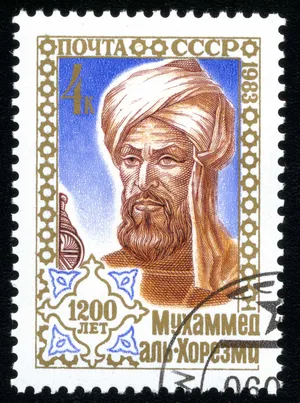
\includegraphics[scale=0.3]{img/Khwarizmi}
 \caption{A stamp of al-Khwarizmi from former USSR in 1983}
 \label{fig:kwarizmi}
\end{figure}

\begin{mdframed}
\index{al-Khwarizmi} \label{sec:Khwarizmi}
Arabic civilization flourished from the beginning of 7th century. Arabic scholars collected and translated the mathematics of Greece, Byzantium, and India after Roman empire collapsed in the 8th century. Al-Mamum became the sixth Caliph and ruled the empire from Baghdad in 813. in 830, he founded an academy called the House of Wisdom where became the center of scientific and philosophy of that time. Al-Manum also built up a library and observatories. Al-Khwarizmi (about 780 - 850 CE, \cref{fig:kwarizmi}) arrived Baghdad in 813; he was one of the famous scholars at the House of Wisdom (\cref{fig:HoW}). We know few details about al-Khwarizmi; even his name looks like a nick name. The prefix `al-' means coming from; it indicates he was native of Khwārizmī, a place in the south of the Aral Sea in central Asia (today belongs partly to Uzbekistan and partly to Turkmenistan).

Al-Khwarizmi worked on elementary algebra. His most famous and important work is the treatise {\em Hisab al-jabr w'al-muqabala} (The Compendious Book on Calculation by Completion and Balancing in 820 CE). It was translated into Latin in the 12th century; its title gives us the word `algebra'. This work is a compilation of rules to find the solutions of linear and quadratic equations. There was no symbolic notations by that time, Instead, al-Khwarizmi systematically presented the rules with intuitive geometric demonstrations. It also contains sections on calculating areas and volumes of geometric figures; al-Khwarizmi also applied algebra to solve them.

His second work (written in 825 CE) introduced Hindu-Arabic numerals and their arithmetic. It was translated to Latin in the same century with the title {\em Liber Algoritmi de numero Indorum} (Al-Khwārizmī Concerning the Hindu Art of Reckoning). From the translation of his name, Algoritmi, in Latin, the word algorithm derives\cite{Britannica-25}.
\end{mdframed}

\begin{figure}[htbp]
 \centering
 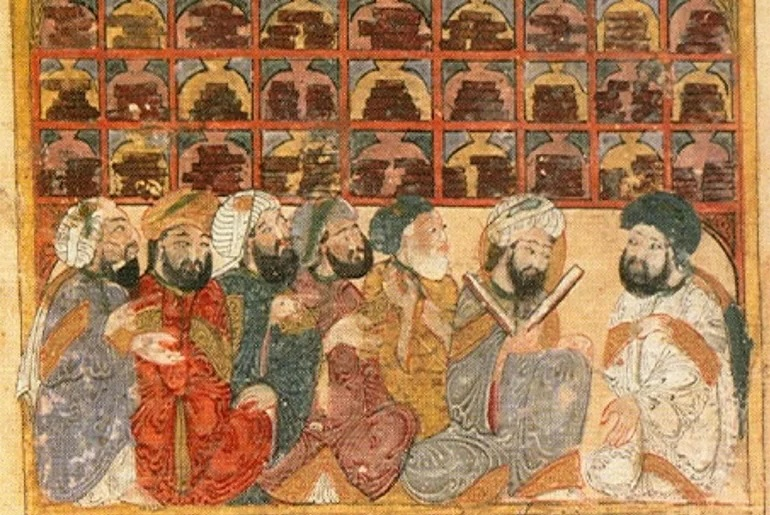
\includegraphics[scale=0.3]{img/HoW}
 \caption{Scholars in library of the `House of Wisdom', Baghdad 1237 CE}
 \label{fig:HoW}
\end{figure}

The decimal positional system has big advantage in computing, particularly when handle big numbers. One can imagine how hard to calculate in Roman numbers, for example, value of MMXXV $-$ CXXXVII, while a primary school kid can find the result like below:

\begin{center}
\opsub[voperator=bottom]{2025}{137}
\end{center}

\label{sec:counting-rods} \index{counting-rods}
This is about subtraction, not to say about multiplication and division. Ancient Chinese mathematicians invented counting rod, a powerful tool, to execute the decimal positional computations despite they lacked of zero in early time (see the previous section). It is a collection of small rods made in bamboo or wood. We don't know the exact time of the invention, but it appeared no later than 1st century CE\footnote{From the document contains the Chinese character 筹 (the term of counting rod) and the related phrases.}. There are two ways to represent a digit: horizontally and vertically as shown in \cref{fig:suanchou-digit}. People use the two arrangements alternatively for each digit to avoid mistakes. If a digit is represented horizontally, then the next digit is vertically. If a digit is zero, then the place is empty without any rods. To make the empty place notable, a special mark of $\square$ or 〇 was invented later. It's easy to compute with counting rods particularly when handling carries: one just needs to put a rod in the place of the next digit as shown in \cref{fig:suanchou-eg}.

\begin{figure}[htbp]
 \centering
 \subcaptionbox{Two ways to represent a number \label{fig:suanchou-digit}}{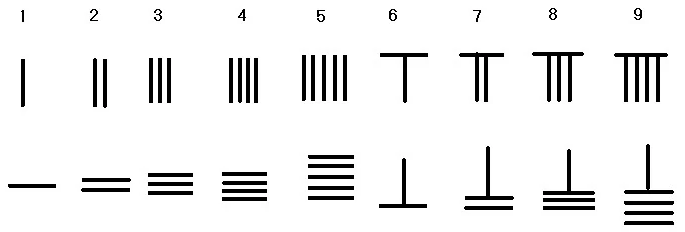
\includegraphics[scale=0.25]{img/suanchou-digit}}
 \subcaptionbox{Example of compute $2025 - 137$ with counting rods \label{fig:suanchou-eg}}{\qquad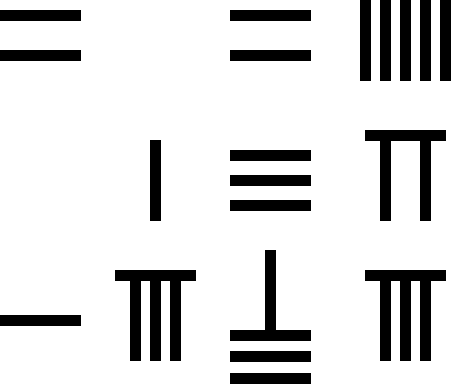
\includegraphics[scale=0.15]{img/suanchou-eg}\qquad}
 \caption{The counting rods}
\end{figure}

\index{Fibonacci}
Only a few intellectuals knew Hindu-Arabic numerals through al-Khwarizmi's work in the 12th century. In 1202, Fibonacci further introduced Hindu-Arabic numerals system to the west through his famous book {\em Liber Abaci} (Book of the Abacus). Interestingly, Fibonacci is also a nickname; the name of this medieval Italian mathematician was Leonardo of Pisa. the nickname came from filius Bonacci in Latin, meaning son of Bonacci. His father held a diplomatic post, whose job was to represent the merchants of the Republic of Pisa who were trading in North Africa and Mediterranean area. Fibonacci learned mathematics from Egyptians, Greeks, Sicilians, and Arabians when travelled widely with his father. He recognized the enormous advantages of Hindu-Arabic numeral system used in the countries he visited. Fibonacci well explained this numeral system in {\em Liber Abaci}, followed with the demonstration of applying the arithmetical operations to many practical problems, such as profit margin, barter, money changing, conversion of weights and measures, partnerships, and interest. It's so popular that was widely copied. It drew the attention of the Holy Roman emperor, Fredrick II, who invited Fibonacci a visit to Pisa in 1225. Fibonacci accepted a challenge from John of Palermo, a scholar of Fredrick's scientific entourage. He successfully solved all problems in the challenge including a cubic equation. By approximation, Fibonacci gave the correct answer up to nine decimal places\cite{Gies-Carney-24}.  The popular number series $1, 1, 2, 3, 5, 8, \dotsc$ is named after Fibonacci, which we'll explain in details in section \ref{sec:Fibonacci-numbers}.

\begin{figure}[htbp]
 \centering
 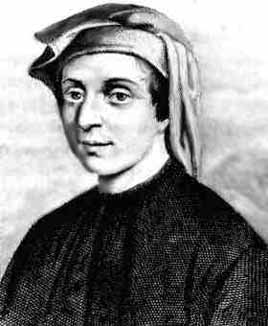
\includegraphics[scale=0.35]{img/Fibonacci}
 \caption{Fibonacci (Leonardo of Pisa), 1175-1250 CE}
 \label{fig:Fibonacci}
\end{figure}

\label{sec:binary-numerals} \index{binary numeral}
More and more intellectuals and merchants spread Hindu-Arabic numeral system worldwide. It becomes a universal human language. German mathematician Leibniz developed another positional numeral system in the 17th century. This 2-based (binary) system led to a revolutionary application in the 20th century; the computer system adopted binary numbers to encode information. With only 0 and 1, binary numbers are much longer than their decimal counterpart. For example, 2025 is 1111 1101 001 in binary format. Despite this, 0/1 can be perfectly modeled as the off/on state of electric device, or low/high level of voltage. Further, 0/1 can map to logical value of false/true, negative/positive result of a test, incorrect/correct answer to a question...all these logical things can be easily handled by machine uniformly as numbers as shown in \cref{tab:binary-arithmatic-logic}.

\begin{table}[htbp]
\[\begin{array}{cccc}
  \begin{tabular}{c|c}
  $x$ & $1-x$ \\
  \hline
  0 & 1   \\
  \hline
  1 & 0   \\
  \end{tabular}
  &
  \begin{tabular}{c|c}
  $x$ & not $x$ \\
  \hline
  false & true  \\
  \hline
  true & false   \\
  \end{tabular}
   \quad & \quad
  \begin{tabular}{c|c|c}
  $x$ & $y$ & $x \times y$ \\
  \hline
  0 & 0 & 0  \\
  \hline
  0 & 1 & 0  \\
  \hline
  1 & 0 & 0  \\
  \hline
  1 & 1 & 1  \\
  \end{tabular}
  &
  \begin{tabular}{c|c|c}
  $x$ & $y$ & $x$ \text{and} $y$ \\
  \hline
  false & false & false \\
  \hline
  false & true & false \\
  \hline
  true & false & false \\
  \hline
  true & true & true \\
  \end{tabular}
\end{array}\]
\captionof{figure}{$1-x$ in binary corresponds to logical not; binary multiplication corresponds to logical and}
\label[figure]{tab:binary-arithmatic-logic}
\end{table}

Our ancestors recognized numbers from counting in daily life and work. People spent more than 4000 years to develop and adopt the modern decimal positional numerals. This is really a long journey. The numeral system wasn't invented by any exact man, nor arose from any civilization in silo. It is a great achievement of all people in the world.

\begin{Exercise}[label={ex:numerals}]
\Question{2025年深圳市南山区小学4年级期末数学考试中出现了这样一道题:“计算$114 \times 21$,同学们用了不同的方法。在思路上这些方法有什么相同的地方?”

\begin{multicols}{2}
\begin{enumerate}
  \renewcommand{\labelenumi}{\textcircled{\theenumi}}
  \item
    \begin{align*}
      114 \times 20 & = 2280 \\
      114 \times 1  & = 114 \\
      2280 + 114 & = 2394
    \end{align*}

  \item
    \begin{align*}
       & 114 \times 21 \\
     = & 114 \times 7 \times 3 \\
     = & 798 \times 3 \\
     = & 2394
    \end{align*}

  \item
    \[\begin{array}{cc}
    \begin{tabular}{|c|c|c|c|}
      \hline
      \times & 100  & 10  & 4 \\
      \hline
      20       & 2000 & 200 & 80 \\
      \hline
      1        & 100  & 10  & 4 \\
      \hline
    \end{tabular}  \quad
    \opadd[voperation=center,
           voperator=bottom]{2280}{114}
    \end{array}\]

  \item
    \opmul[displayshiftintermediary=all,
           voperator=bottom,
           voperation=top]{114}{21}
    \oplput(1,-2){$\cdots$ \opmul[style=text]{114}{1}}
    \oplput(1,-3){$\cdots$ \opmul[style=text]{114}{20}}
\end{enumerate}
\end{multicols}
这四个方法中,哪些利用了十进制位值制计数系统的优势?
}

\Question{可以利用$n = a_m b^m + a_{m-1} b^{m-1} + \cdots + a_a b + a_0$进行进制转换:
  \begin{enumerate}[1)]
    \item 用$n$除以$b$得到余数$a_0$、商$q_0$。
    \item 把$n$替换为$q_0$,再次用$n$除以$b$得到余数$a_1$、商$q_1$。
    \item 把$n$替换为$q_1$,重复上述步骤直到商$q_m = 0$。
  \end{enumerate}
  则$n$的$b$进制表示为$a_m \cdots a_1a_0$。请将十进制数123转换为(a)玛雅文;(b)古巴比伦文;(c)计算机二进制表示。
}

\Question{$\bigstar$\footnote{标星号的题目较难。}如果你会编程,请用自己熟悉的语言实现二进制到十进制的相互转换。}

\Question{$\bigstar$证明一个数的位值制表示是唯一的。提示:考虑如果一个数有两种表示会怎样? \label{qn:unique-pos-rep}}
\end{Exercise}

\begin{Answer}[ref={ex:numerals}]
\Question{ \textcircled{1}、\textcircled{3}、\textcircled{4} }

\Question{将十进制数123转换为(a)玛雅文;(b)古巴比伦文;(c)计算机二进制表示。

玛雅文:

\begin{align*}
123 \div 20 &= 6 \cdots 3 & \underline{\ \circ \ } \\
6 \div 20 &= 0 \cdots 6   & \circ \circ \circ \\
120 &= 6 (20) + 3  &  \text{从上到下6、3}
\end{align*}

古巴比伦文:YY YYY
\begin{align*}
123 \div 60 &= 2 \cdots 3 \\
2 \div 20 &= 0 \cdots 2   \\
120 &= 2 (60) + 3
\end{align*}

计算机二进制表示:1111011
\begin{align*}
123 \div 2 &= 61 \cdots 1 &
61 \div 2 &= 30 \cdots 1   &
30 \div 2 &= 15 \cdots 0 \\
15 \div 2 &= 7 \cdots 1 &
7 \div 2 &= 3 \cdots 1 &
3 \div 2 &= 1 \cdots 1 \\
1 \div 2 &= 0 \cdots 1 & & & &
\end{align*}
}

\Question{编程实现二进制到十进制的相互转换。

\begin{center}
 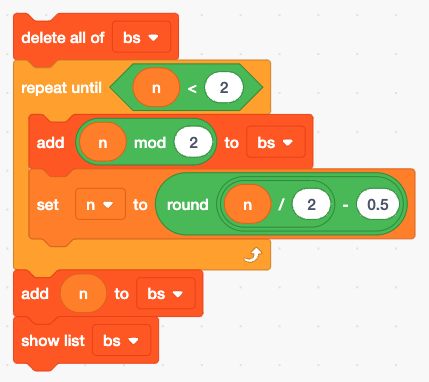
\includegraphics[scale=0.3]{img/scratch-bin}
 \qquad
 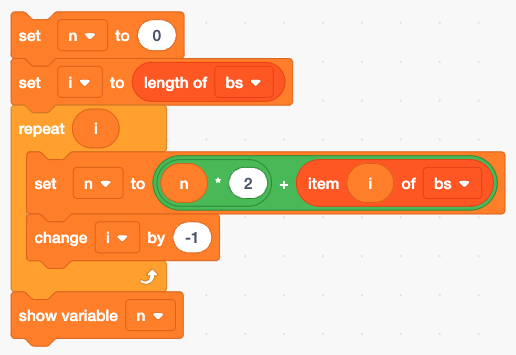
\includegraphics[scale=0.3]{img/scratch-dec}
 \captionof{figure}{Scratch例子程序:十进制$n$与二进制$bs$相互转换,左:$10 \to 2$;右:$2 \to 10$}
 \label{fig:bin-dec-scratch}
\end{center}

说明:\lstinline|round|是四舍五入。对$n/2$ - 0.5四舍五入相当于对$n/2$取整,求得$n$除以2的除数。$bs$中的二进制数字低位在前,高位在后。下面是对应的Python例子程序:

\begin{lstlisting}[language=Python, frame=single]
def bin(n):
    bs = []
    while n > 1:
        bs = [n % 2] + bs
        n = n // 2
    return [n] + bs

def dec(bs):
    n = 0
    for b in bs:
        n = n*2 + b
    return n
\end{lstlisting}

与Scratch和Python的循环不同,下面的Haskell例子给出了递归实现。其中的二进制数字高位在前、低位在后。

\begin{Haskell}[frame=single]
bin x = if x < 2 then [x] else (bin (x `div` 2)) ++ [x `mod` 2]
dec = foldl (\n x -> n*2 + x) 0
\end{Haskell}
}

\Question{证明一个数的位值制表示是唯一的。

\begin{proof}
假设一个数还有另一个表示。如果它们的位数不同,我们在较短的前面添加0,使它们一样长。令补0后的表示分别为$a_{m} a_{m-1} \cdots a_1 a_0$和$c_m c_{m-1} \cdots c_1 c_0$。按照\cref{eq:pos-rep}计算的值相等,即:
\[
  a_m b^m + a_{m-1} b^{m-1} + \cdots + a_1 b + a_0 = c_m b^m + c_{m-1} b^{m-1} + \cdots + c_1 b + c_0
\]

将$a_0$和$c_0$移到右边,剩下的移到左边:

\[
  (a_m - c_m) b^m + (a_{m-1} - c_{m-1}) b^{m-1} + \cdots + (a_1 - c_1) b = c_0 - a_0
\]

左边可以被$b$整除,所以$c_0 - a_0$也可以被$b$整除。由于$c_0$、$a_0$都只能是0到$b - 1$的整数,所以它们的差只能是$1 - b, \dots , -1, 0, 1, \dots b - 1$中的一个。但其中只有0能被$b$整除。所以$c_0 - a_0 = 0$,即$c_0 = a_0$。

接下来$(a_m - c_m) b^m + (a_{m-1} - c_{m-1}) b^{m-1} + \cdots + (a_1 - c_1) b = 0$。由于$b \neq 0$,两边除以$b$,然后将$a_1$和$c_1$移动到左边:

\[
  (a_m - c_m) b^m + (a_{m-1} - c_{m-1}) b^{m-1} + \cdots + (a_2 - c_2) b = c_1 - a_1
\]

同样可以推出$c_1 = a_1$。重复这个步骤$m$次,最后得到$a_m = c_m$。这就证明了两种表示是一样的,即位值制表示是唯一的。
\end{proof}
}
\end{Answer}

\ifx\wholebook\relax \else
\section{Answer}
\shipoutAnswer

\section{Greek alphabet} \label{ch:greek-letters}
\subimport{inc/}{greek-zh-cn}


 \begin{table}[htbp]
     \centering
     \begin{tabular}{|c|c|c||c|c|c|}
         \hline
               \textbf{Upper} & \textbf{Lower} & \textbf{Pronunciation} & \textbf{Upper} & \textbf{Lower} & \textbf{Pronunciation} \\
         \hline
         A         & $\alpha$    & Alpha &      N         & $\nu$         & Nu \\
         B         & $\beta$     & Beta &       $\Xi$         & $\xi$         & Xi \\
         $\Gamma$  & $\gamma$    & Gamma &      O    & o    & Omicron \\
         $\Delta$  & $\delta$    & Delta &      $\Pi$         & $\pi$         & Pi \\
         E         & $\epsilon$  & Epsilon &    P        & $\rho$        & Rho \\
         Z         & $\zeta$     & Zeta &       $\Sigma$      & $\sigma$      & Sigma \\
         H         & $\eta$      & Eta &        T        & $\tau$        & Tau \\
         $\Theta$  & $\theta$    & Theta &      Y    & $\upsilon$    & Upsilon \\
         I         & $\iota$     & Iota &       $\Phi$        & $\phi$        & Phi \\
         K         & $\kappa$    & Kappa &      X        & $\chi$        & Chi \\
         $\Lambda$ & $\lambda$   & Lambda &     $\Psi$        & $\psi$        & Psi \\
         M         & $\mu$       & Mu &         $\Omega$      & $\omega$      & Omega \\
         \hline
     \end{tabular}
     \caption{Greek alphabet}
     \label{tab:greek-alphabet}
 \end{table}

\begin{thebibliography}{99}
\subimport{inc/}{bib-zh-cn}
\end{thebibliography}

\expandafter\enddocument
\fi
